\section{Task definition}
\label{sec:task}

We define melody transcription as the task of converting a music recording into a \emph{monophonic} (non-overlapping) sequence of \emph{notes} which constitute its melody.\footnote{Melody is difficult to precisely define---here we adopt an implicit definition based on a dataset of crowdsourced melody annotations.} Given a music recording $\bm{a}$ of length $T$, our task is to 
%generate 
uncover 
the sequence of $N$ notes~${\bm{y} = [\bm{y}_1,\dots,\bm{y}_N}]$ that represent the melody of $\bm{a}$.  For many MIR tasks, including transcription, it can be convenient to work with \emph{features} of audio ${\bm{X} = \texttt{Featurize}(\bm{a})}$, rather than the raw waveform $\bm{a}$. 
Hence, a melody transcription algorithm is a procedure that maps featurized audio to notes, i.e.~${\bm{y} = \texttt{Transcribe}(\bm{X})}$. 

% CHRIS: Cut for space but may be useful to someone
% \begin{figure}
%     \centering
%     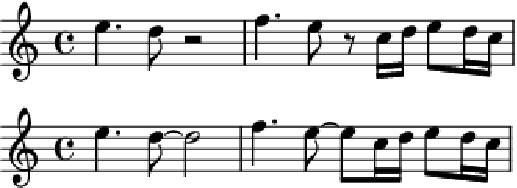
\includegraphics[width=8.1cm]{figs/heuristic_offsets.pdf}
%     \caption{
% The same note onsets engraved with ground truth~(top) vs. heuristic~(bottom) offsets. 
% We argue that onset prediction suffices for producing melody transcriptions that are both recognizable and readable. 
% }
%  \label{fig:heuristic_offsets}
% \end{figure}

Canonically, a musical note consists of an onset time, a musical pitch, and an offset time. 
However, in this work  
%(and as in~\cite{laaksonen2014automatic}) 
we disregard offsets and define a note to be a pair $\bm{y}_i = (t_i,n_i)$ consisting of an onset time~${t_i \in [0,T)}$ and discrete musical pitch~${n_i \in \mathbb{V} = \{\text{A0}, \ldots, \text{C8}\}}$.
We ignore offsets for 
%three 
two reasons. 
First, accurate offsets have been found to be considerably less important for human perception of transcription quality compared to accurate onsets~\cite{ycart2020investigating}. 
Second, in our dataset,
a heuristically-determined offset is identical to the ground truth offset for $89\%$ of notes.\footnote{The heuristic we adopt sets the offset of one note equal to the onset of the next, i.e., it assumes the melody is legato.}
% Finally, we argue intuitively that onsets and pitches suffice for both recognizing and reading melodies---see~\Cref{fig:heuristic_offsets} for an example.

Formally, a musical audio recording of length~$T$ seconds sampled at rate~$f_s$ is a vector~${\bm{a} \in \mathbb{R}^{Tf_s}}$. 
A featurization of audio ${\bm{X} \in \mathbb{R}^{Tf_k \times d}}$ is a matrix of $d$-dimensional features of audio, sampled uniformly at some rate ${f_k \ll f_s}$ (for example, $\bm{X}$ could be a spectrogram).
Intuitively, the function ${\texttt{Featurize} : \mathbb{R}^{Tf_s} \to \mathbb{R}^{Tf_k \times d}}$ defined by ${\bm{a} \mapsto \bm{X}}$ maps 
raw audio to a feature representation more conducive to learning. 
A melody of length $N$ is a sequence of notes 
$\bm{y} = [\bm{y}_1,\dots,\bm{y}_N] \in \mathbb{Y}^N$
consisting of onset-pitch pairs ${\bm{y}_i = (t_i,n_i)} \in \mathbb{Y} = \mathbb{R}^+ \times \mathbb{V}$ where ${t_i < t_j}$ if ${i < j}$. Given a featurization $\bm{X}$, the melody transcription task is to construct a transcription algorithm ${\texttt{Transcribe} : \mathbb{R}^{Tf_k \times d} \to \mathbb{Y}^N}$ such that ${\bm{X} \mapsto \bm{y}}$.

\subsection{Evaluation}
\label{sec:eval}

To evaluate a melody transcription method $\texttt{Transcribe}$, 
we adopt a standard metric commonly used for evaluation in polyphonic music transcription tasks, namely,  ``onset-only notewise F-measure''~\cite{ycart2020investigating}. 
This metric scores an estimated transcript $\texttt{Transcribe}(\bm{X})$ by first matching its note onsets to those in the reference $\bm{y}$ with $50$ms of tolerance, and then computes a standard \fone{} score where an estimated note is treated as correct if it is the same pitch as its matched reference note. 
This ``notewise'' metric represents a departure from the ``frame-based'' metrics typically used to evaluate melody extraction algorithms---Ycart~et~al.\ demonstrate in~\cite{ycart2020investigating} that this particular notewise metric correlates more strongly with human perception of transcription quality than any other common metric, including frame-based ones.

We make a slight modification to this notewise metric 
specific to the melody transcription setting: an estimate $\texttt{Transcribe}(\bm{X})$ may receive full credit if it is off by a fixed octave shift but otherwise identical to the reference. 
In downstream settings, melody transcriptions are likely to be used in an octave-invariant fashion, e.g.,~they may be shifted to read more comfortably in treble clef, or performed by singers with different vocal ranges. 
Hence, we modify the evaluation criteria by simply taking the highest score over octave shifted versions of the estimate:
\begin{equation*}
    \max_{\sigma \in \mathbb{Z}} \texttt{\fone}(\texttt{OctaveShift}(\texttt{Transcribe}(\bm{X}), \sigma), \mathbf{y}).
\end{equation*}
Henceforth, we refer to this octave-invariant metric as \fone. 